% !TEX TS-program = pdflatex
% !TEX encoding = UTF-8 Unicode

% This is a simple template for a LaTeX document using the "article" class.
% See "book", "report", "letter" for other types of document.

\documentclass[11pt]{article} % use larger type; default would be 10pt

\usepackage[utf8]{inputenc} % set input encoding (not needed with XeLaTeX)

%%% Examples of Article customizations
% These packages are optional, depending whether you want the features they provide.
% See the LaTeX Companion or other references for full information.

%%% PAGE DIMENSIONS
\usepackage{geometry} % to change the page dimensions
\geometry{a4paper} % or letterpaper (US) or a5paper or....
% \geometry{margin=2in} % for example, change the margins to 2 inches all round
% \geometry{landscape} % set up the page for landscape
%   read geometry.pdf for detailed page layout information

\usepackage{graphicx} % support the \includegraphics command and options

% \usepackage[parfill]{parskip} % Activate to begin paragraphs with an empty line rather than an indent

%%% PACKAGES
\usepackage{booktabs} % for much better looking tables
\usepackage{array} % for better arrays (eg matrices) in maths
\usepackage{paralist} % very flexible & customisable lists (eg. enumerate/itemize, etc.)
\usepackage{verbatim} % adds environment for commenting out blocks of text & for better verbatim
\usepackage{cite}
% These packages are all incorporated in the memoir class to one degree or another...

%%% HEADERS & FOOTERS
\usepackage{fancyhdr} % This should be set AFTER setting up the page geometry
\pagestyle{fancy} % options: empty , plain , fancy
\renewcommand{\headrulewidth}{0pt} % customise the layout...
\lhead{}\chead{}\rhead{}
\lfoot{}\cfoot{\thepage}\rfoot{}

%%% SECTION TITLE APPEARANCE
\usepackage{sectsty}
\allsectionsfont{\sffamily\mdseries\upshape} % (See the fntguide.pdf for font help)
% (This matches ConTeXt defaults)

\usepackage{authblk} %Allow more complex author information

%%% ToC (table of contents) APPEARANCE
\usepackage[nottoc,notlof,notlot]{tocbibind} % Put the bibliography in the ToC
\usepackage[titles,subfigure]{tocloft} % Alter the style of the Table of Contents
\usepackage{subfig} % make it possible to include more than one captioned figure/table in a single float
\usepackage{amsmath}
\renewcommand{\cftsecfont}{\rmfamily\mdseries\upshape}
\renewcommand{\cftsecpagefont}{\rmfamily\mdseries\upshape} % No bold!

%%% END Article customizations

%%% The "real" document content comes below...

\title{A Game Theoretical Exploration of Open Science}
\author[1]{Robert Olendorf}
\author[2]{Steve Koch}
\affil[1]{University Libraries, University of New Mexico}
\affil[2]{Department of Physics and Astronomy, University of New Mexico}
%\date{} % Activate to display a given date or no date (if empty),
         % otherwise the current date is printed 

\begin{document}
\maketitle

%\section{}

The value of sharing data and other research products is increasingly recognized. Many funding agencies, such as NSF and NIH now require that data created through their grants be made available to others in a reasonable amount of time. Additionally, many journals now require or encourage that the data used as a basis for a manuscript be made available. Universities, including University of New Mexico, are working to create data repositories to help researchers make the products of their research available. 

While acknowledging the public good of making their data more avaialble, many if not most individual researchers are still reluctant to make their data available. There are several reasons for this attitude. First and foremost is researchers fear that others will publish from their data before them. Additionally, researchers worry that their data will be used without proper attribution and that their data will be misunderstood or used inappropriately. Essentially, researchers believe that while making their data more open may benefit society, there are few personal benefits and considerable personal risks to doing so. This dichotomy between the wish to make research more open for the public good, and to keep data closed for personal interest creates a tension between funding agencies, policy makers and others hoping to make research more open, and individual researchers who create the content.

In this manuscript we will use game theoretical arguments, specifically work based on the well researched Prisoners' Dilemma to explore how we can create an atmosphere where researchers feel they receive direct benefits to making their data more open. We will show that it is possible that even in the current environment openness in research direclty benefits researchers. We will also explore ways to further increase direct benefits to researchers. Finally, we will provide examples from our own experiences in open research, as well as experimental examples from the literature that show how openness can be encouraged.
\section{Theory}
\subsection{The Prisoners' Dilemma and Open Science}
\begin{figure}[ht]
	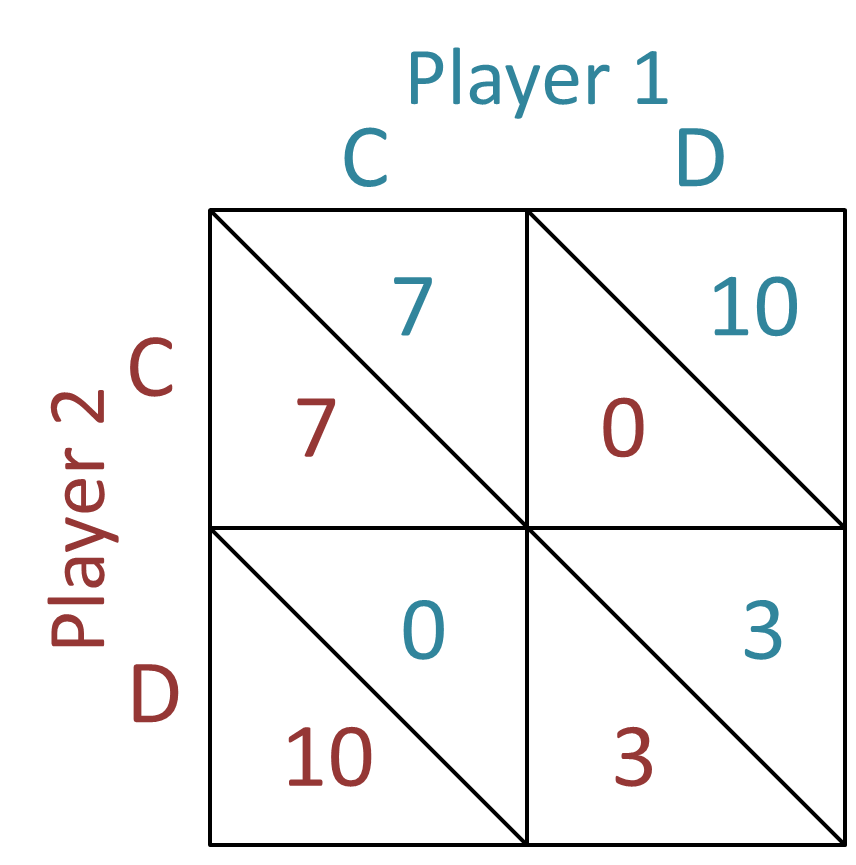
\includegraphics[width=0.5\textwidth]{pdmatrix.png}
	\caption{A sample example matrix for the Prisoners' Dilemma. The players can either Cooperate(C) or Defect(D).  Numbers above the diagonal represent payoffs to Player 1, numbers below the diagonal represent payoffs to Player 2.}
	\label{pdmatrix}
\end{figure}
We will use the Prisoners' Dilemma to explore open science. The Prisoners' Dilemma is a game theoretical construct developed in the RAND corporation by Merrill Flood and Melving Dresher in 1950 \cite{ABAGFBEC19920101, unm.b196052419570101} to study situations where there is both a strong incentive to cooperate, but also a strong temptation to defect. Figure~\ref{pdmatrix} shows a specific example of the Prisoners' Dilemma (PD). In the PD each player can do one of two actions, Cooperate, or Defect (cheat). Mutual cooperation yields a relatively high reward. However, if a player can defect while the other player cooperates, they get an even higher reward (the big payoff) the other player gets the lowest possible payoff (the suckers payoff). There are a few constraints on the payoff matrix. The big payoff to a Defector against a Cooperator needs to be higher than mutual cooperation. If mutual cooperation is higher, then cooperating is always favored. Second, mutual cooperation must be higher than the average of the big payoff and the sucker's payoff. In the example shown in Figure~\ref{pdmatrix}, the payoff for mutual cooperation is seven, while the average of the big pay off and the sucker's payoff is 5 ((10+0)/2). This prevents an alternating strategy from being favored in the Iterated Prisoners' Dilemma discussed below.

If the game is to be played only once, then the only rational move is to defect. If Player 1 knows that Player 2 will cooperate, then she maximizes her reward by defecting and yielding 10. On the other hand, if Player 1 knows that Player 2 will defect, then she should still defect because then she will get at least 3 rather than 0. Player 2 follows the same logic and the equilibrium is for both players to defect. This is known as a Nash Equilibrium, defined as a situation when neither player benefits by changing strategies \cite{unm.b196052419570101}.

The Prisoners' Dilemma serves as a useful paradigm for exploring open research for a number of reasons. First, is often the model used to explore situations where individuals must trade personal gain for a public good. More importantly, if as we will argue, that open research presents both personal rewards as well as risks, this model captures this dynamic.

\subsection{Tit-For-Tat}
If the game is to played for some unknown number of times (Iterated Prisoners' Dilemma or IPD), then the situation becomes much more complicated because the players are now able to base their decisions both on past behavior and expectations of future behavior. It is important that the number of interactions is not known to the players, otherwise the last interaction is played just like a single play Prisoners' Dilemma and both players defect. Since both players know that the last move is to defect, they use similar logic on the second to last interaction, continuing until the first interaction where both players defect.

 In 1981  Axelrod and Hamilton \cite{axelrodhamilton1981} conducted a tournament where strategies for playing the IPD were pitted agains one another. Surprisingly, the simplest submission won, Tit-For-Tat (TFT). The TFT strategy cooperates on the first move than simply repeats the other player's last move thereafter. Subsequent analysis and tournaments suggest that TFT is successful because of three traits. First it is nice in that in cooperates by default. Second, it is retaliatory, in defects if the other player defects. Finally, it is forgiving because it cooperates if the other player then cooperates on future moves. Subsequent work has shown that other successful strategies also share these traits
\cite{axelroddion1988, ABAGFBEC19920101, unm.b685148920000101}.
\subsection{Population Dynamics}
In most cases players are not just playing agains one player, but exist in a population of players. We must therefore consider the dynamics of strategies in the IPD played against a population of strategies. To do this we must redefine our equlibrium from a situation where neither player benefits by changing strategies to the situation where a population of players, cannot be invaded by any alternative strategy that is initially rare. This is known as an Evolutionarily Stable Strategy (ESS) first developed by J. Maynard Smith \cite{smithprice1973}. An ESS is actually a Nash equilbirium extended for In the case of a population rather than two individuals. 

\begin{figure}[ht]
	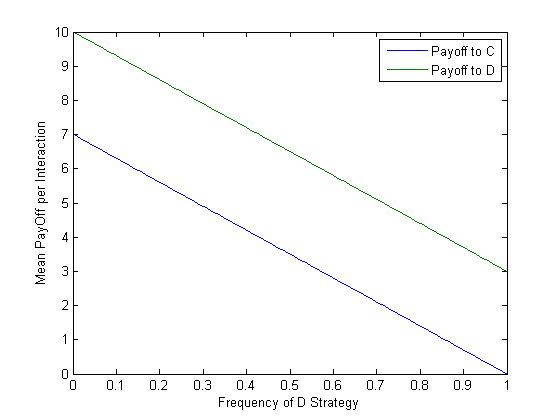
\includegraphics[width=0.7\textwidth]{c_vs_d.png}
	\caption{The payoffs to Cooperate and Defect strategies as a function of the frequency of Defectors in the population.}
	\label{cvsd}
\end{figure}

We can determine the expected payoff for each interaction to each strateg with the following formulas. We use the payoff per interaction to allow us to compare between long and short expected numbers of interactions.
\begin{subequations}
	\begin{equation}
	\omega_{D} = \frac{\mu * (1-F_{D})(P_{CD}) + F_{D } * P_{DD}}{\mu}
	\end{equation}
\mbox{ cancels out so the pay off is independent of the number of times the players expect to interact.}
	\begin{equation}
	\omega_{D} = (1-F_{D})(P_{CD}) + F_{D } * P_{DD}
	\label{d_in_dvsc}
	\end{equation}
\end{subequations}
and likewise, the expected payoff to Cooperating is
\begin{equation}
	\omega_{C} = (1-F_{D})(P_{CC}) + F_{D } * P_{DC}
	\label{c_in_dvsc}
\end{equation}
where $\mu$ is the expected number of times players play the game together, $\omega_{x}$ is the expected payoff to strategy x, $ F_{x}$ is the frequency of strategy x in the population and $P_{XY}$ is the pay off to Player Y when the othe Player plays X.  In the simple case of a Cooperators and Defectors we can see in Figure~\ref{cvsd} that while the expected payoff to both strategies decreases as the number of defectors increases.Also, both strategies achieve a higher payoff in an environment with more Cooperators, but because Defectors always achieve a higher payoff the population is only stable with pure defection. This is essentially the same result as we saw with only two players.

\begin{figure}[ht!]
	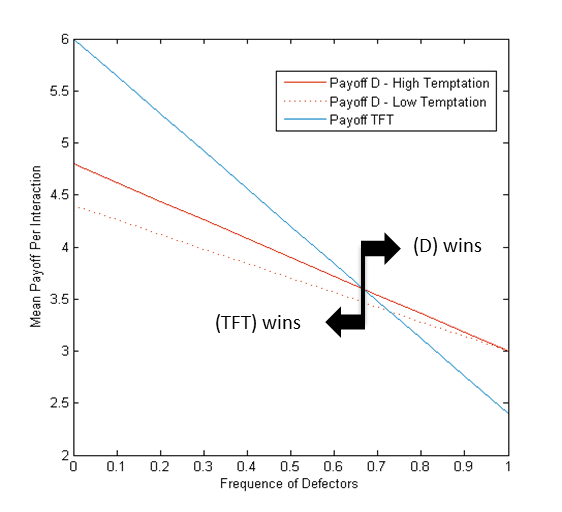
\includegraphics[width=0.7\textwidth]{tftvsdannotated.png}
	\caption{The payoffs to TFT and Defect as a function of the frequency of Defectors in the population.}
	\label{tftvsd}
\end{figure}

We approach the determining the payoffs in a similar way, the payoff to Defecting in a population of Defectors and TFT players is
\begin{equation}
	\omega_{D} = \frac{(1-F_{D} *  P_{CD} +F_{D} *  (\mu - 1) * P_{DD})}{\mu}
	\label{d_in_dvstft}
\end{equation}
and  the payoff to TFT is
\begin{equation}
	\omega_{D} = \frac{1-F_{D} *P_{CC} + F_{D} * (P_{DC} + (\mu - 1) * P_{DD}}{\mu}
	\label{tft_in_dvstft}
\end{equation}
There are a number of things to notice. First, as shown in Figure~\ref{tftvsd}, Defectors are not always favored. When the TFT line is above the Defectors line, TFT is favored and eventual come to dominate the population at equilibrium. The point where the lines cross is a threshold point where if the frequency of Defectors is less than this point, TFT will be favored and come to dominate, while if the frequency of Defectors is higher than this point, Defectors are favored. This derives from two factors. First, while Defectors enjoy a long string of high payoffs against Cooperators, they only enjoy this high payoff once against TFT strategists. Similarly, TFT strategists only suffer the suckers payoff once against a Defector, while a Cooperator endures a potentially long string of suckers payoffs. 

\begin{figure}[ht]
	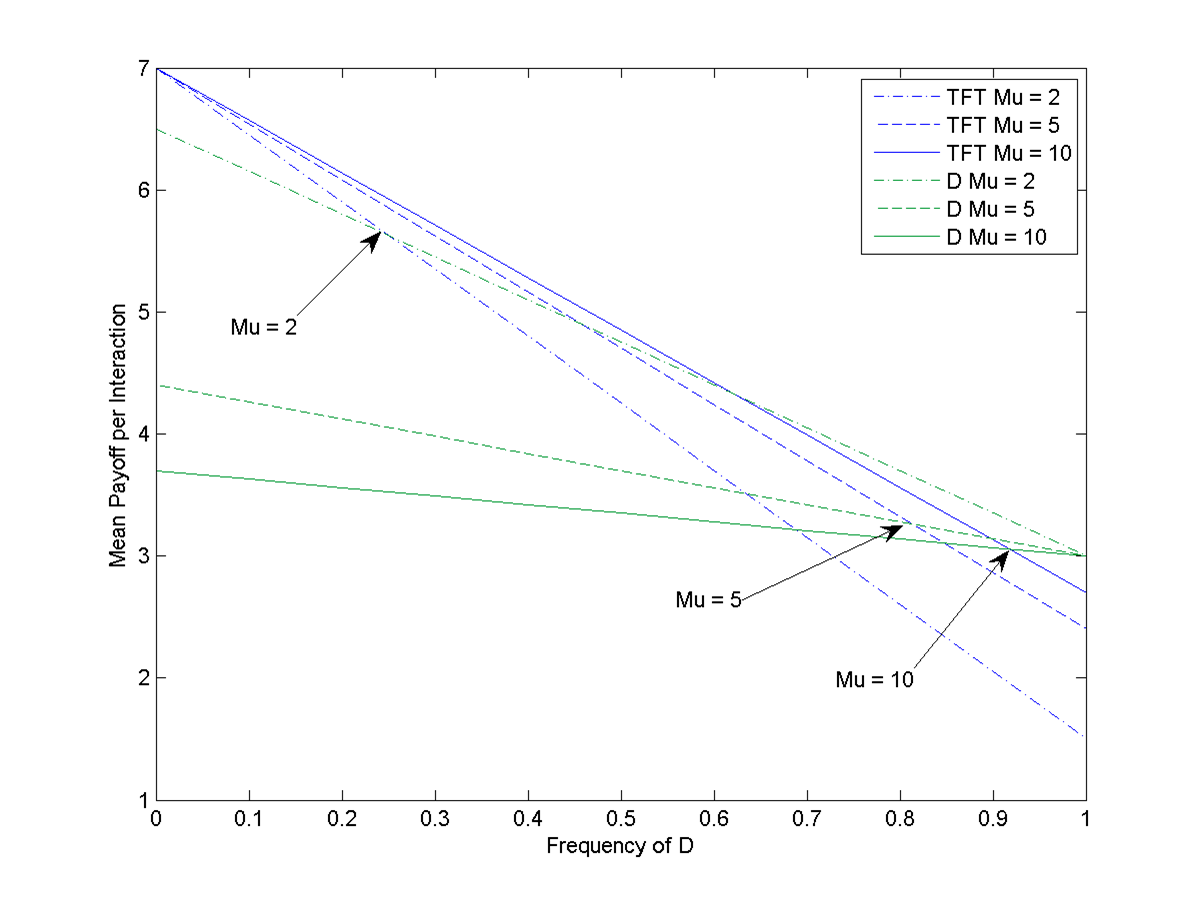
\includegraphics[width=0.7\textwidth]{payoffvsmu.png}
	\caption{The affect of increasing expected interaction length in TFT versus D populations.}
	\label{muintft}
\end{figure}

Extending this affect is the influence the expected interaction length has on the threshold point.  Figure~\ref{muintft}, shows how with very short expected interaction lengths, the threshold for Defectors to dominate is very low, while increasing the expected interaction length rapidly increases this threshold. This results from the fact that Defectors only get one big payoff on their first interaction with a TFT. Thereafter, both TFT and Defectors defect realizing a relatively low payoff. At the same time, TFT only get the suckers payoff once, and thereafter get the low, but still higher, mutual defection payoff. The longer two players interact, the less important the initial payoff becomes to each player and the affect of the mutual defection payoff dominates the mean payoff.

Also, as shown in Figure~ref{tftvsd} the temptation to defect (the payoff to a player when she defects while the other player cooperates) influences this threshold. The higher the temptation to defect, the lower the threshold value is meaning that Defectors are favored at a lower frequency. Also, while the expected number of interactions with another player was not an issue when Defectors and Cooperators were competing ($\mu$ cancels out in equations~\ref{d_in_dvsc} and \ref{c_in_dvsc}), the expected number of interactions is a factor when TFT and Defectors compete. 

\section{Analysis}
We will now turn to using this body of theory to explore how open research functions now and more importantly how researchers, institutions, funding agencies, journals and other interested parties can modify their behaviors to favor a more open environment in research. While, all of these people and institutions probably agree that increased sharing of data, ideas and other products of research benefits science and society, researchers are far less convinced that they can benefit directly. Conversely, most researchers probably feel that opening up their research is a net cost for them and if they do practice a more open philosphy its for the good of society rather than their own benefit.


\bibliographystyle{plain}

\bibliography{refs}
\end{document}
